\documentclass[conference]{IEEEtran}
\IEEEoverridecommandlockouts
\usepackage{cite}
\usepackage{amsmath,amssymb,amsfonts}
\usepackage{graphicx}
\usepackage{textcomp}
\usepackage{xcolor}
\usepackage{booktabs}
\usepackage{url}
\renewcommand{\topfraction}{0.95}
\renewcommand{\bottomfraction}{0.95}
\renewcommand{\textfraction}{0.05}
\renewcommand{\floatpagefraction}{0.9}
\renewcommand{\dbltopfraction}{0.95}
\renewcommand{\dblfloatpagefraction}{0.9}
\def\BibTeX{{\rm B\kern-.05em{\sc i\kern-.025em b}\kern-.08em
    T\kern-.1667em\lower.7ex\hbox{E}\kern-.125emX}}

\begin{document}

\title{Clause-Activation Signatures (CAS) for Attack-Family Attribution in IoMT}

\author{\IEEEauthorblockN{Anonymous Author(s)}
\IEEEauthorblockA{\textit{Affiliation withheld for review}\\
email@example.com}}

\maketitle

\begin{abstract}
Intrusion detection for the Internet of Medical Things (IoMT) needs more
than a correct label: a forensic analyst needs a compact, auditable reason
for each attribution. We study Clause-Activation Signatures (CAS) ---
per-class sets of Tsetlin Machine (TM) clauses selected by
complementary-pairs stability selection (CPSS) from the clause-activation
space of a trained weighted TM, with an error-control bound on spurious
inclusions. On CICIoMT2024 (WiFi/MQTT, family level), verified across three
independently seeded TMs, CAS attribution improves over the raw
weighted-vote TM it is extracted from: macro-F1 $0.765 \pm 0.029$ vs.\
$0.692 \pm 0.004$ at the verified operating point, using only 39--58
sign-positive clauses per family out of a 2{,}400-clause pool. The
signatures carry an exact identifiability certificate: they form a maximally
5-disjunct code on every seed --- any mixture of up to five of the six
families is exactly decodable from the union of their signatures (100\%
noiseless; 99.8--100\% at 5\% noise with the correct thresholded decoder,
which collapses to $\sim$1\% under the strict decoder). In a binary
normal-vs-attack reduction, the attack signature lifts ranking quality over
the base TM (AUROC 0.940 vs.\ 0.819, three seeds). We also report two
negative results without smoothing: open-set novelty power is weak under
correct conformal false-flag control, and cross-retraining signature
identity is near chance because clause indices are seed-dependent. CAS is
best understood as an interpretability-and-attribution layer with
statistical certificates that can also denoise a mediocre base detector.
\end{abstract}

\begin{IEEEkeywords}
Tsetlin Machine, interpretable machine learning, intrusion detection, IoMT,
stability selection, disjunct codes, attack attribution, open-set
recognition
\end{IEEEkeywords}

\section{Introduction}
Machine-learned intrusion detection for the Internet of Medical Things
(IoMT) carries a dual requirement: detections must be correct, and they must
be \emph{explainable} in a form a forensic analyst can act on, because the
defended systems can directly affect patient safety. Post-hoc explainability
(SHAP, LIME, Anchors) dominates the IDS literature but explains one
black-box prediction at a time, with no stability guarantee: retrain the
model, or perturb the explainer, and the explanation changes.

The Tsetlin Machine (TM)~\cite{granmo2018} is an attractive base learner:
its unit of computation --- a conjunctive clause over Boolean literals ---
is human-readable by construction, and its weighted variant~\cite{phoulady2020}
retains this property. Recent work shows TMs are competitive IoMT
detectors~\cite{jaiswal2026iomt}. But a trained TM's clauses are numerous,
noisy, and seed-dependent: of 400 clauses learned per class, which genuinely
characterize an attack family, and how many could be spurious?

We study \textbf{Clause-Activation Signatures (CAS)}: for each class $\ell$,
select the clauses whose activation is \emph{stably} predictive of $\ell$
via complementary-pairs stability selection (CPSS)~\cite{shah2013} over the
clause-activation space; split the selection by coefficient sign into
inculpatory (evidence for) and exculpatory (evidence against) sets; and
report the Shah--Samworth bound on the expected number of false inclusions.
Attribution is signature matching: a flow is attributed to the family whose
signature it best matches.

\textbf{Contributions.}
(1) A correctness-audited, fully seed-reproducible CAS implementation on
TMU~\cite{tmu} clause activations, including a sign-filtering fix without
which the attribution scorer is worse than random (\S\ref{sec:cpss}).
(2) A three-seed verified result on CICIoMT2024: CAS beats its base TM by
$+0.07$ macro-F1, robust at stability threshold $\pi_{\mathrm{thr}} \ge 0.7$
but not at the default 0.6, where CPSS-internal randomness swings macro-F1
by up to 0.13 (\S\ref{sec:taska}); $B{=}15$ vs.\ $25$ subsamples makes no
material difference, and fusing CAS with the raw TM vote adds nothing.
(3) Signed, human-readable evidence lists per family with an explicit
error-control certificate, reported as loose where it is loose
(\S\ref{sec:signatures}).
(4) An exact disjunct-code certificate: CAS signatures are maximally
5-disjunct on all seeds, with mixture-decoding simulation isolating the
decoder, not the code, as the noise bottleneck (\S\ref{sec:disjunct}).
(5) A binary normal-vs-attack reduction lifting attack-detection AUROC from
0.819 to 0.940 (\S\ref{sec:binary}).
(6) Two negative results reported plainly: weak open-set novelty power under
correct conformal false-flag control (\S\ref{sec:taskb}), and near-chance
cross-seed signature identity (\S\ref{sec:stability}).

\section{Related Work}
\textbf{Tsetlin Machines.} The TM~\cite{granmo2018} learns conjunctive
clauses over Boolean literals via bandit-driven Type~I/II feedback; the
weighted TM~\cite{phoulady2020} learns an integer vote weight per clause.
TM-based IDS goes back to rule extraction on KDD'99/NSL-KDD~\cite{abeyrathna2020};
recently Jaiswal et al.~\cite{jaiswal2026iomt} trained TMs on CICIoMT2024
(reported 90.7\% six-class accuracy; F1 averaging unspecified and
hyperparameter tables not machine-readable in the preprint) and on
MedSec-25~\cite{jaiswal2026medsec} (macro-F1 97.8\%). That work explains
individual predictions by the clauses that fired; it does not aggregate
clause activations into per-family signatures with error control --- the gap
CAS addresses.

\textbf{Stability selection.} Meinshausen and B\"uhlmann~\cite{meinshausen2010}
introduced stability selection; Shah and Samworth's CPSS~\cite{shah2013}
bounds the expected number of falsely selected variables without assumptions
on the selector. We apply CPSS to \emph{clause activations} rather than raw
features. To our knowledge, stability selection has not previously been
combined with Tsetlin Machines nor used for clause-level forensic signatures
in security; we frame this as methodological transfer --- the guarantee
quantifies selection stability, not detection accuracy.

\textbf{Disjunct codes.} $t$-disjunct matrices from group
testing~\cite{du1993} give identifiability: if no column's support is
covered by any union of $t$ others, any $\le t$-sparse mixture is exactly
decodable. We compute this certificate exactly for the CAS signature
incidence matrix and evaluate strict (COMP) and thresholded noisy decoders
by simulation.

\textbf{IDS dataset validity.} Our dataset choice follows standard validity
criteria~\cite{sommer2010,engelen2021,arp2022}: CICIoMT2024~\cite{dadkhah2024}
is, to date, the only peer-reviewed, widely adopted, IoMT-specific,
multi-protocol benchmark, and its published flow schema contains no IP/port
fields, removing the most common leakage channel by design. A published
critique~\cite{domenech2025} of its windowing and splitting is addressed in
\S\ref{sec:discussion}.

\textbf{Interpretable IDS.} Post-hoc SHAP/LIME explanations of black-box IDS
dominate (e.g.,~\cite{xaiids2025}). Intrinsically interpretable,
stability-vetted rule \emph{sets} per attack family --- the object CAS
produces --- appear absent from the literature; we make this claim with the
usual absence-of-evidence caveat.

\section{Method: Clause-Activation Signatures}
\subsection{Booleanization and base detector}
Each numeric flow feature is discretized into 10 quantile bins
(KBinsDiscretizer, edges fit on train only) and encoded as cumulative
thermometer bits (``feature $\ge$ bin $k$''); TMU handles literal negation
internally. A data-quality fix mattered: the \texttt{Rate} feature contained
$+\infty$ values from near-zero-duration flows, collapsing quantile binning
to a degenerate bin; clipping to the finite train max raised macro-F1 from
$\sim$0.54 to $\sim$0.72. A weighted multiclass TM (400 clauses/class,
$T=320$, $s=8.0$, weighted clauses, 25 epochs) is trained on six classes.

\subsection{Clause-activation space}
Running flows through the trained TM yields $Z \in \{0,1\}^{n \times 2400}$
(6 classes $\times$ 400 clauses): $Z[x,j]=1$ iff clause $j$ fires on $x$.
CAS operates entirely in this space --- a flow is represented by
\emph{which rules match it}.

\subsection{CPSS signature extraction, with a necessary sign fix}
\label{sec:cpss}
For each family $\ell$ (one-vs-rest), CPSS repeats $B$ times: split a
validation half of the test set into complementary halves, fit
$\ell_1$-regularized logistic models of $\ell$-vs-rest on $Z$ across
$C \in$ geomspace$(0.001, 0.1, 6)$, and record whether each clause was
selected at any grid point. The stability score $\hat{\pi}_j$ is the
selection fraction over the $2B$ half-fits; the signature is
$S_\ell = \{j : \hat{\pi}_j \ge \pi_{\mathrm{thr}}\}$. The $C$ grid was
empirically restricted to the range that actually induces sparsity on this
clause pool; wider grids inflated the union-over-grid support and made the
certificate vacuous. All CPSS fits use a fixed liblinear random seed, making
extracted signatures exactly reproducible.

\textbf{Threshold sensitivity (finding).} $\pi_{\mathrm{thr}}$ is not a
benign knob at its default: at $\pi_{\mathrm{thr}}{=}0.6$ the attribution F1
varied by up to 0.13 under re-seeded CPSS fits on the same trained TM, while
at $\pi_{\mathrm{thr}} \ge 0.7$ results are stable. The mechanism is visible
in the $\hat{\pi}$ distribution: many clauses sit just below/above 0.6, so
borderline inclusion noise dominates; at 0.8 the selected set is stably
separated. We report $\pi_{\mathrm{thr}} = 0.8$ as the verified operating
point.

\textbf{Sign filtering (correctness fix).} CPSS selects on
$|\text{coefficient}| > 0$ --- correct for the error-control bound, wrong
for attribution: a stably \emph{negative} coefficient is evidence
\emph{against} $\ell$. Naively summing $\hat{\pi}_j z_j(x)$ over the
sign-agnostic $S_\ell$ produced an attribution scorer at macro-F1 $= 0.004$,
worse than random. We track each clause's mean signed coefficient and use
$S_\ell^{+} = \{j \in S_\ell : \overline{\mathrm{coef}}_j > 0\}$
(inculpatory) and $S_\ell^{-}$ (exculpatory) for scoring, while the
certificate applies to the full sign-agnostic $S_\ell$ --- a stated scoping
gap.

\textbf{Attribution score.}
\begin{equation}
s_\ell(x) = \frac{\sum_{j \in S_\ell^{+}} \hat{\pi}_j z_j(x) - \sum_{j \in S_\ell^{-}} \hat{\pi}_j z_j(x)}{\sum_{j \in S_\ell^{+}} \hat{\pi}_j},
\end{equation}
with $\hat{y} = \arg\max_\ell s_\ell(x)$.
Normalization by the inculpatory weight is required: unnormalized scores
scale with signature size, not match quality.

\subsection{Error-control certificate}
With $q_\Lambda$ estimated as $\mathrm{mean}(\hat{\pi}) \cdot p$,
$E[V] \le q_\Lambda^2 / ((2\pi_{\mathrm{thr}} - 1) p)$, $p = 2400$. We
report these bounds as loose where they are loose (\S\ref{sec:signatures}):
they certify that most of each signature is likely real, not that it is
near-noise-free.

\section{Experimental Setup}
\textbf{Dataset.} CICIoMT2024~\cite{dadkhah2024}, WiFi/MQTT branch,
family-level labels (Benign, DDoS, DoS, MQTT, Recon, Spoofing), 22 numeric
flow features. Stratified caps for tractability: $\le$40{,}000 train /
$\le$15{,}000 test rows per family (Benign 19{,}291 and Spoofing 16{,}047
used in full), giving 195{,}338 train / 80{,}868 test rows. The raw
distribution is heavily imbalanced (DDoS+DoS $\approx$ 95.7\% of
flows~\cite{dadkhah2024}); we report macro-F1 and per-class metrics
throughout.

\textbf{Protocol.} Signatures are built (CPSS) on a random half of the test
set and evaluated on the disjoint other half --- no leakage between
signature fitting and evaluation. Multi-seed results use three independently
trained TMs (seeds 42, 7, 123) with fully seeded CPSS.

\section{Results}
\subsection{Task A --- closed-set family attribution}
\label{sec:taska}
Table~\ref{tab:headline} gives the verified headline. (i) At
$\pi_{\mathrm{thr}}{=}0.8$ CAS beats its base detector on every seed
(per-seed: 0.792/0.778/0.726 vs.\ TM 0.686/0.697/0.693) with \emph{smaller}
signatures than lower thresholds. (ii) $\pi_{\mathrm{thr}}{=}0.6$ is
unstable: the recorded primary run scored 0.776 there, but re-seeded CPSS at
the same threshold and same trained model scores as low as 0.638.
(iii) Fusion with the raw TM vote adds nothing over CAS alone at 0.8.

\begin{table}[t]
\centering
\caption{Task A: verified three-seed macro-F1 on CICIoMT2024.}
\label{tab:headline}
\begin{tabular}{lcc}
\toprule
Method & $B{=}15$ & $B{=}25$ \\
\midrule
Weighted-TM argmax (base) & $0.692 \pm 0.004$ & (same models) \\
CAS $\pi_{\mathrm{thr}}{=}0.6$ & $0.688 \pm 0.032$ & $0.678 \pm 0.028$ \\
CAS $\pi_{\mathrm{thr}}{=}0.7$ & $0.743 \pm 0.015$ & $0.737 \pm 0.022$ \\
\textbf{CAS $\pi_{\mathrm{thr}}{=}0.8$} & $\mathbf{0.765 \pm 0.029}$ & $0.750 \pm 0.034$ \\
CAS $\pi_{\mathrm{thr}}{=}0.9$ & $0.762 \pm 0.038$ & $0.761 \pm 0.038$ \\
Fusion (TM + CAS, $\lambda$ on val) & $0.764 \pm 0.010$ & $0.768 \pm 0.013$ \\
\bottomrule
\end{tabular}
\end{table}

\begin{table}[t]
\centering
\caption{Recorded primary run (seed 42, $\pi_{\mathrm{thr}}{=}0.6$, $B{=}25$):
per-family precision/recall/F1. One draw, kept for per-family detail.}
\label{tab:perfamily}
\begin{tabular}{lcc}
\toprule
Family & TM P / R / F1 & CAS P / R / F1 \\
\midrule
Benign   & 0.72 / 0.30 / 0.43 & 0.72 / \textbf{0.64} / \textbf{0.68} \\
DDoS     & 0.86 / 0.77 / 0.81 & 0.91 / 0.73 / 0.81 \\
DoS      & 0.78 / 0.89 / 0.83 & 0.76 / 0.92 / 0.83 \\
MQTT     & 0.63 / 0.75 / 0.68 & 0.78 / 0.89 / \textbf{0.83} \\
Recon    & 0.82 / 0.90 / 0.86 & 0.97 / 0.89 / \textbf{0.93} \\
Spoofing & 0.41 / 0.69 / 0.52 & \textbf{0.55} / 0.61 / \textbf{0.58} \\
\bottomrule
\end{tabular}
\end{table}

Table~\ref{tab:perfamily} and Fig.~\ref{fig:cm} (top) give per-family detail from
the recorded primary run. The largest gains land where the base detector is
weakest: Benign recall $0.30 \rightarrow 0.64$ and Spoofing precision
$0.41 \rightarrow 0.55$. DDoS/DoS mutual confusion persists in both methods
--- a documented, dataset-inherent property~\cite{domenech2025}, not a
signature-quality artifact.

\begin{figure*}[t]
\centering
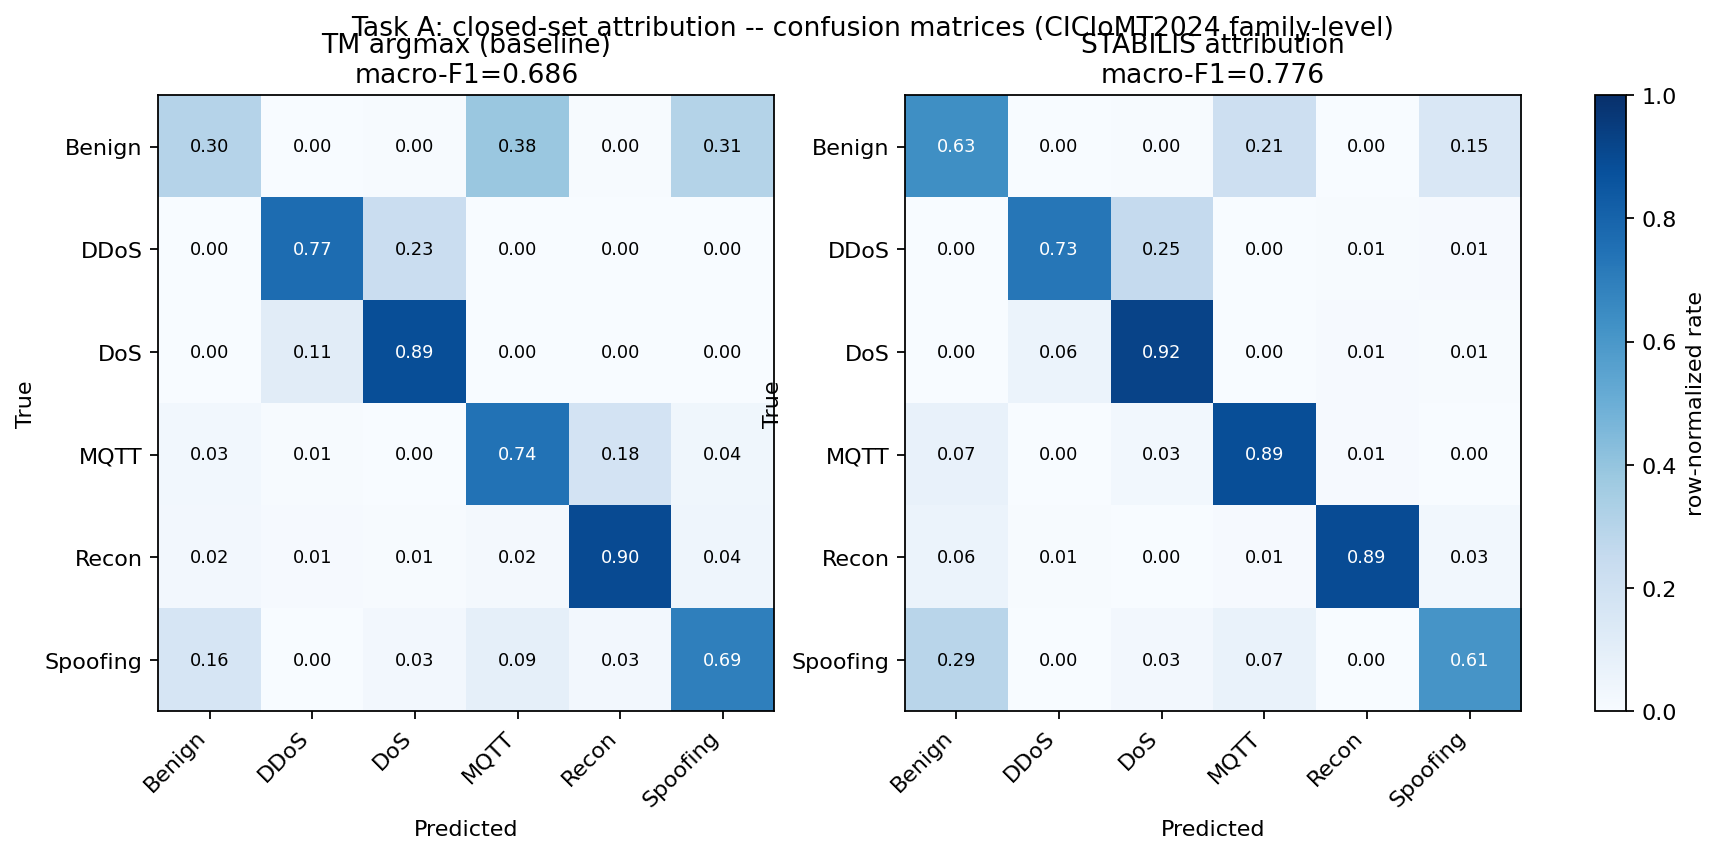
\includegraphics[width=0.70\textwidth]{figs/task_a_confusion_matrices.png}\\[4pt]
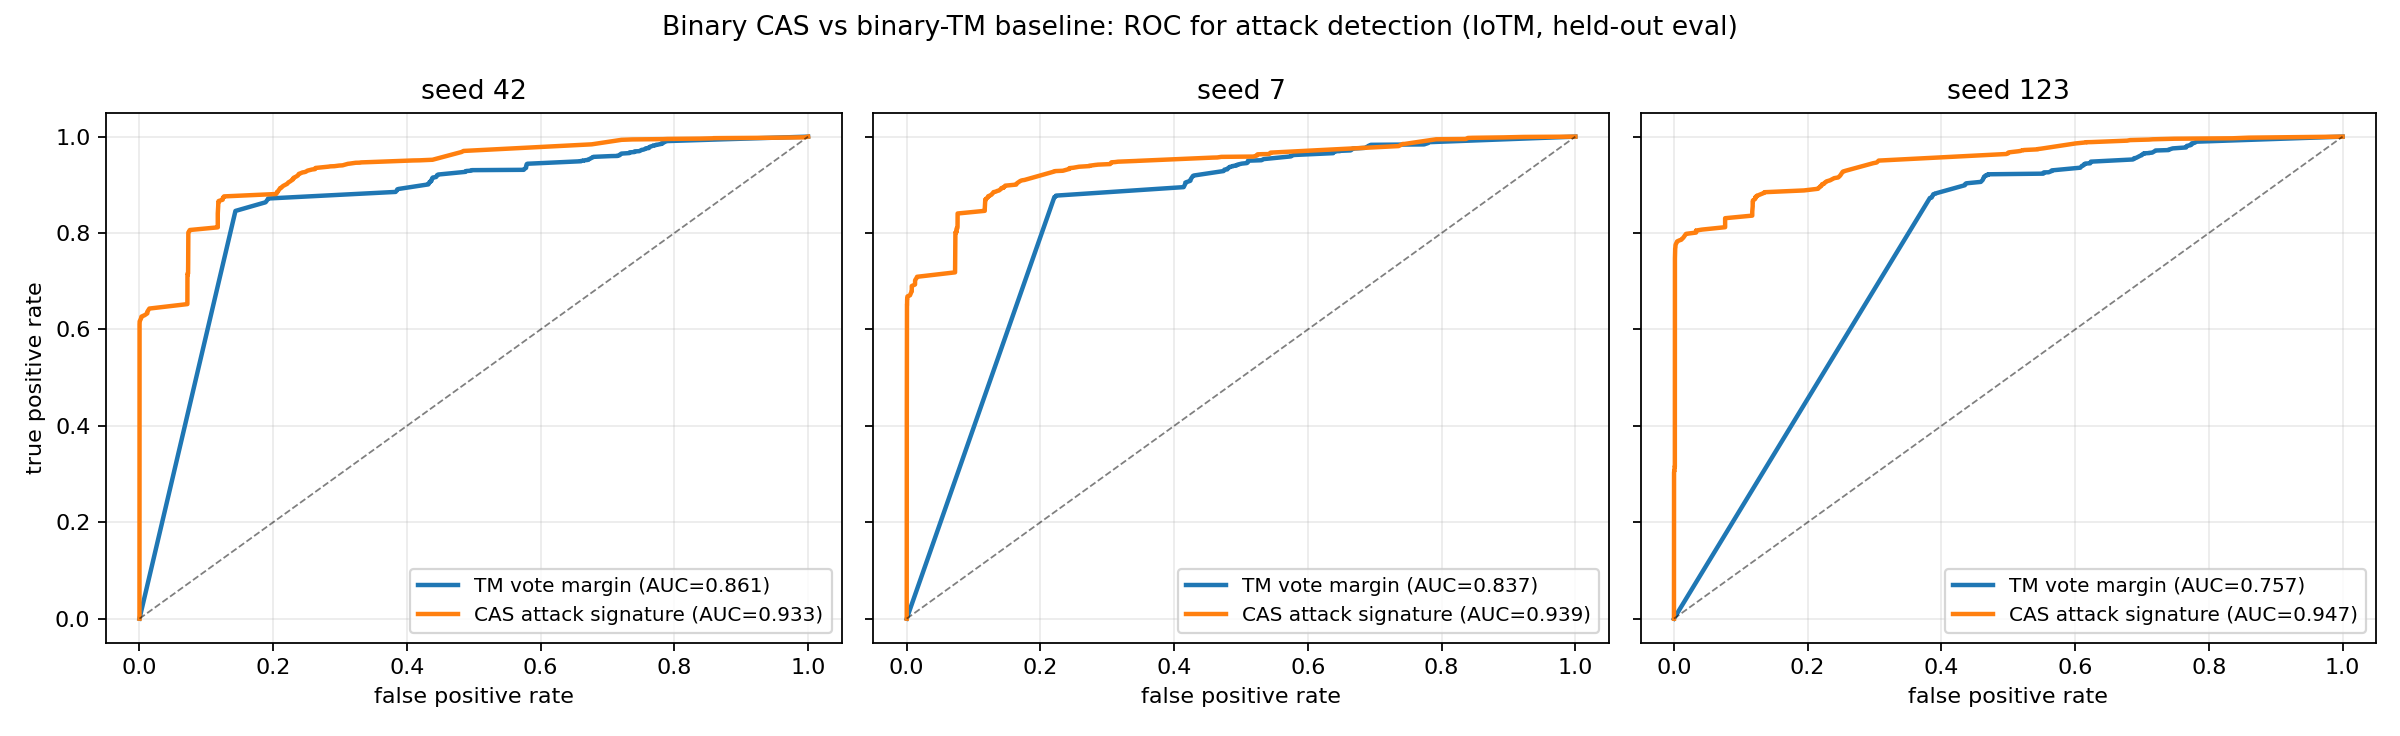
\includegraphics[width=0.58\textwidth]{figs/binary_cas_roc_iotm.png}
\caption{\textbf{Top:} closed-set attribution confusion matrices
(row-normalized), recorded primary run: weighted-TM argmax baseline (left)
vs.\ CAS attribution (right); the Benign diagonal improves from 0.30 to
0.63, MQTT from 0.74 to 0.89. \textbf{Bottom:} ROC for attack detection in
the binary reduction, three independently seeded binary TMs --- CAS
attack-signature score vs.\ the TM's own vote margin; the signature score
dominates on every seed (AUC 0.933/0.939/0.947 vs.\ 0.861/0.837/0.757).}
\label{fig:cm}
\label{fig:roc}
\end{figure*}

\subsection{Signature content and certificates}
\label{sec:signatures}
Recorded primary run ($\pi_{\mathrm{thr}}{=}0.6$): certified $|S|$ /
attribution $|S^{+}|$ / $E[V]$ per family --- Benign 216/48/${\le}165$;
DDoS 131/55/${\le}98$; DoS 289/42/${\le}212$; MQTT 167/58/${\le}72$; Recon
115/29/${\le}82$; Spoofing 311/56/${\le}250$. At the verified
$\pi_{\mathrm{thr}}{=}0.8$ operating point, attribution signatures shrink to
a mean of 39--47 sign-positive clauses per family while F1 \emph{improves}
--- compaction and accuracy are not in tension here (Fig.~\ref{fig:pithr}).
Decoded attack-signature clauses are forensically legible: high-rate and
SYN-flag conjunctions dominate the inculpatory list (median one literal per
clause, e.g., \texttt{Rate $\ge$ bin4}; \texttt{syn\_flag\_number $\ge$
bin1}), while long low-rate benign-profile conjunctions dominate the
exculpatory list --- consistent with the flooding-dominated attack mix.

\begin{figure}[t]
\centering
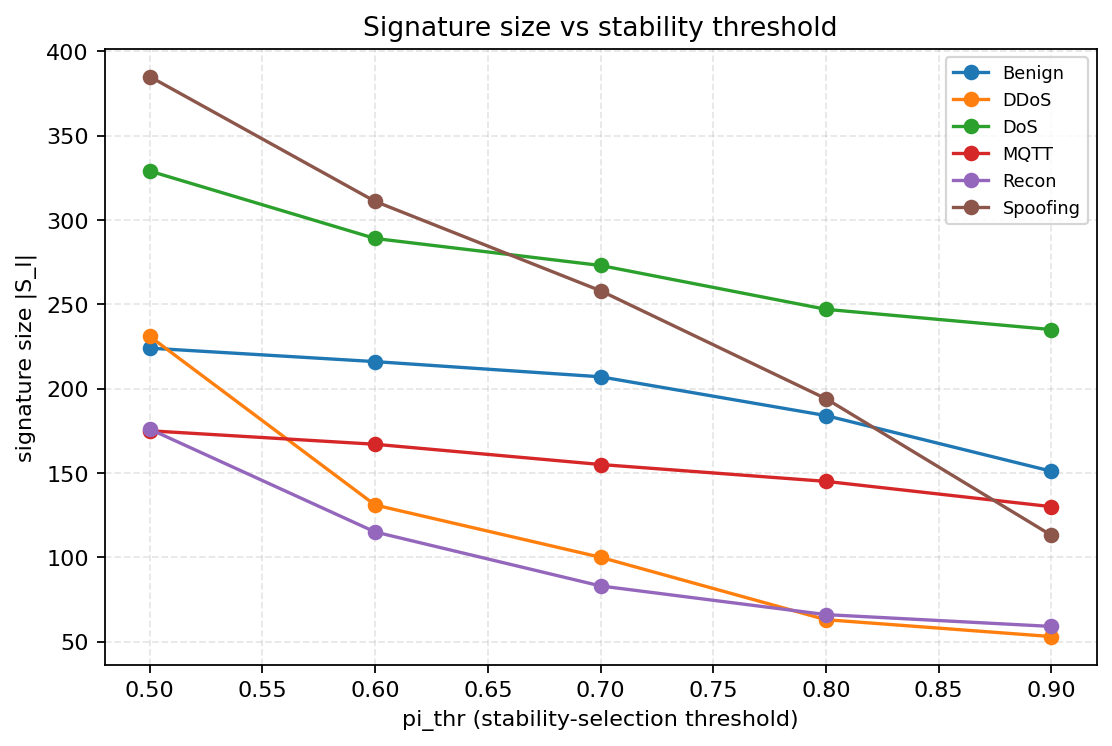
\includegraphics[width=0.62\columnwidth]{figs/pi_thr_sweep.png}
\caption{Signature size vs.\ stability threshold $\pi_{\mathrm{thr}}$ per
family. The accuracy-optimal operating point is 0.8
(Table~\ref{tab:headline}), not the default 0.6.}
\label{fig:pithr}
\end{figure}

\subsection{Binary reduction --- the attack signature}
\label{sec:binary}
Collapsing the five attack families into one \textsc{attack} class and
training a dedicated 2-class TM (same hyperparameter family) yields a single
normal-vs-attack CAS (three seeds, held-out eval):
Table~\ref{tab:binary} and Fig.~\ref{fig:roc} (bottom). The base
binary TM over-predicts attack (recall 0.988 at precision 0.847); the attack
signature rebalances to a better operating point and a much stronger ranking
(it concentrates true-normal flows near score 0, where the TM margin leaks
mid-range mass --- the source of the AUROC gap). (Data-state note: the binary arm uses a 5-bin re-binarization of
the same flows; the per-class arm uses 10 bins. Both are self-consistent.)

\begin{table}[t]
\centering
\caption{Binary attack detection, three seeds (mean).}
\label{tab:binary}
\begin{tabular}{lccc}
\toprule
Method & attack F1 & R / P & AUROC \\
\midrule
Binary TM argmax & $0.912 \pm 0.000$ & 0.988 / 0.847 & 0.819 \\
\textbf{CAS attack signature} & $\mathbf{0.928 \pm 0.007}$ & 0.910 / 0.947 & \textbf{0.940} \\
\bottomrule
\end{tabular}
\end{table}

\subsection{Task B --- open-set behavior (leave-one-family-out)}
\label{sec:taskb}
Holding out one family entirely, retraining, rebuilding signatures, and
calibrating a per-predicted-family split-conformal novelty threshold at
target $\epsilon = 0.05$ (two folds): Spoofing --- FPR 0.035, TPR 0.040,
AUROC 0.275; MQTT --- FPR 0.027, TPR 0.081, AUROC 0.622. The conformal
false-flag guarantee holds (both FPRs under target, as finite-sample theory
promises), but detection power against genuinely novel families is weak ---
for Spoofing below chance. For Spoofing there is a forensic reading:
ARP-spoofing traffic shares transport-layer characteristics with legitimate
ARP-based device discovery, so it does not present as novel in this
22-feature space --- a measured blind spot of this detector family, worth
reporting as such.

\subsection{Signature identifiability --- DISJUNCT certificates}
\label{sec:disjunct}
Treating the six families' inculpatory signatures as columns of a binary
incidence matrix, we compute the exact $t$-disjunctness certificate (brute
force over the other five columns --- exact at this scale) and simulate
$t{=}2$ mixture decoding (500 random family pairs; $z$ = OR of their
signature columns, plus independent bit-flip noise), three seeds,
$\pi_{\mathrm{thr}} \in \{0.6, 0.8\}$ (Table~\ref{tab:disjunct}). The
signatures are not merely predictive --- they are an \emph{identifiable
code}: any mixture of up to five of the six families is exactly decodable
noiselessly, on every seed, without any overlap-reduction step. Under noise
the binding constraint is the \emph{decoder}, not the code: strict COMP
collapses immediately, exactly as the method specification warns, while the
thresholded decoder restores near-perfect decoding at 5\% noise.

\begin{table}[t]
\centering
\caption{DISJUNCT certificates (all seeds, both $\pi_{\mathrm{thr}}$).}
\label{tab:disjunct}
\begin{tabular}{lc}
\toprule
Result & Value \\
\midrule
$\hat{t}$ (disjunctness) & \textbf{5 (maximal, 6 families)} \\
Clauses removed by overlap reduction & 11--22 \\
Noiseless mixture decoding, strict COMP & \textbf{100\%} \\
5\% noise, strict COMP & 0.2--1.8\% \\
5\% noise, thresholded COMP @0.9 & 85--90\% \\
5\% noise, thresholded COMP @0.8 & \textbf{99.8--100\%} \\
15\% noise, thresholded COMP @0.8 & 68--76\% \\
\bottomrule
\end{tabular}
\end{table}

\subsection{Cross-seed stability --- a negative result}
\label{sec:stability}
Across three independently seeded TMs, pairwise Kuncheva index on raw
signature clause-index overlap is near zero per family ($-0.015$ to $0.111$).
CAS stabilizes selection \emph{within} a trained
TM --- which is what Task A relies on --- but clause $\#47$ of one seed's
Benign bank and clause $\#47$ of another's are unrelated learned rules, so
cross-retraining signature identity does not hold at the index level; a
clause-content alignment step is future work. We report the negative result
because a ``forensic signature'' claim without it would overclaim.

\section{Discussion}
\label{sec:discussion}
\textbf{When does CAS add value?} CAS beat its base TM exactly when the base
detector had slack: IoTM's base is mediocre (0.69) and CAS denoises it; on a
near-ceiling base the same construction is lossy compression (two companion
datasets were evaluated and demoted for this reason). CAS is therefore best
deployed as an \emph{attribution and auditing layer} --- compact signed
evidence with certificates --- that may also improve the decision when the
base is weak.

\textbf{Answering the published critique.} Dom\'enech~\cite{domenech2025}
shows CICIoMT2024 models can suffer large cross-dataset F1 drops; our claims
are accordingly single-dataset and our conformal FPR control is calibrated
in-distribution --- cross-dataset CAS transfer is open, not claimed.

\textbf{Limitations.} (i) Single-dataset evidence (deliberate, per the
selection rationale). (ii) No post-hoc XAI baseline (SHAP/Anchors)
comparison --- the most direct test of the interpretability claim ---
remains future work. (iii) $E[V]$ bounds are loose.
(iv) $\pi_{\mathrm{thr}}{=}0.6$ instability (\S\ref{sec:cpss}) is mitigated
by operating at 0.8, but its cause (borderline $\hat{\pi}$ mass) deserves
study. (v) Cross-seed signature identity is weak (\S\ref{sec:stability}).
(vi) DISJUNCT decoding is validated on synthetic OR-mixtures, not real
multi-family traffic (absent from the dataset).

\section{Conclusion}
Clause-Activation Signatures turn a trained Tsetlin Machine's noisy clause
pool into compact, signed, per-family evidence lists with two certificates:
a statistical bound on spurious inclusions, and an exact disjunctness
guarantee that the signatures are identifiable under mixture. Verified
across three seeds on CICIoMT2024, they improve closed-set attribution over
the base detector ($0.765$ vs.\ $0.692$ macro-F1) and yield a stronger
binary attack detector (AUROC 0.940), while failing instructively (open-set
power, cross-seed identity) where a ``signature'' cannot promise more ---
for IoMT forensics, that honesty is the point.

\begin{thebibliography}{15}
\bibitem{granmo2018} O.-C. Granmo, ``The Tsetlin Machine --- a
game-theoretic bandit-driven approach to optimal pattern recognition with
propositional logic,'' \emph{arXiv:1804.01508}, 2018.
\bibitem{phoulady2020} O.-C. Granmo and S. Phoulady, ``The Weighted Tsetlin
Machine,'' \emph{arXiv:2002.01245}, 2020.
\bibitem{jaiswal2026iomt} R. Jaiswal, P.-A. Andersen, L. R. Cenkeramaddi,
L. Jiao, and O.-C. Granmo, ``A Tsetlin Machine-driven Intrusion Detection
System for Next-Generation IoMT Security,'' \emph{IEEE SVCC} /
\emph{arXiv:2604.03205}, 2026.
\bibitem{shah2013} R. Shah and R. Samworth, ``Variable selection with error
control: another look at stability selection,'' \emph{JRSS-B}, vol. 75,
no. 1, pp. 55--80, 2013.
\bibitem{tmu} O.-C. Granmo et al., ``TMU: Tsetlin Machine Unified,''
github.com/cair/tmu.
\bibitem{abeyrathna2020} K. D. Abeyrathna et al., ``Intrusion Detection
with Interpretable Rules Generated using the Tsetlin Machine,'' \emph{IEEE
SSCI}, 2020.
\bibitem{jaiswal2026medsec} R. Jaiswal et al., ``On-Device Interpretable
Tsetlin Machine-Based Intrusion Detection for Secure IoMT,''
\emph{arXiv:2605.16707}, 2026.
\bibitem{meinshausen2010} N. Meinshausen and P. B\"uhlmann, ``Stability
selection,'' \emph{JRSS-B}, vol. 72, no. 4, pp. 417--473, 2010.
\bibitem{sommer2010} R. Sommer and V. Paxson, ``Outside the Closed World: On
Using Machine Learning for Network Intrusion Detection,'' \emph{IEEE S\&P},
2010.
\bibitem{engelen2021} G. Engelen, V. Rimmer, and W. Joosen,
``Troubleshooting an Intrusion Detection Dataset: the CICIDS2017 Case
Study,'' \emph{IEEE SPW}, 2021.
\bibitem{arp2022} D. Arp et al., ``Dos and Don'ts of Machine Learning in
Computer Security,'' \emph{USENIX Security}, 2022.
\bibitem{dadkhah2024} S. Dadkhah et al., ``CICIoMT2024: A benchmark dataset
for multi-protocol security assessment in IoMT,'' \emph{Internet of Things},
vol. 28, art. 101351, 2024.
\bibitem{domenech2025} J. Dom\'enech Fons, ``Evaluating and enhancing
intrusion detection systems in IoMT: The importance of domain-specific
datasets,'' \emph{Internet of Things}, 2025.
\bibitem{xaiids2025} ``Explainable AI for Interpreting ML-based IDS using
LIME and SHAP,'' \emph{Applied Sciences}, vol. 15, no. 13, 2025.
\bibitem{du1993} D.-Z. Du and F. K. Hwang, \emph{Combinatorial Group Testing
and Its Applications}, World Scientific, 1993.
\end{thebibliography}

\end{document}
